\documentclass[11pt, addpoints, answers]{exam}

\usepackage{amsmath, amssymb}
\usepackage{xcolor}
\usepackage{tikz}
\usepackage{enumerate}
\usepackage{graphicx}
\usepackage{tabularx}
\usepackage{algorithm}
\usepackage{algpseudocode}

\usepackage{graphics}
\usepackage{tikz}
\usepackage{tikz-qtree}
\usepackage{drawstack}

\usetikzlibrary{graphs}
\tikzset{every tree node/.style={minimum width=2em,draw,circle},
    blank/.style={draw=none},
    edge from parent/.style=
    {draw,edge from parent path={(\tikzparentnode) -- (\tikzchildnode)}},
    level distance=1.2cm}

\newcommand{\red}[1]{\textcolor{red}{#1}}
\newcommand{\blue}[1]{\textcolor{blue}{#1}}

% For inserting code snippets.
\usepackage{listings}
\lstset{
    columns = fixed,
    basewidth = {0.5em},
    breaklines = true,
    backgroundcolor = \color{white},
    keywordstyle = \color[RGB]{40, 40, 255},
    numberstyle = \footnotesize\color{darkgray},
    commentstyle = \ttfamily\color{violet},
    basicstyle = \ttfamily,
    stringstyle = \ttfamily\color[RGB]{128, 0, 0},
    showstringspaces = false,
    language = {[11]C++},
    escapechar = \@
}
\lstnewenvironment{cpp}[1][]{\lstset{language = {[11]C++}, #1}}{}

\renewcommand{\baselinestretch}{1.15}
\setlength{\parskip}{1.25\baselineskip}

% headers, footers, titles
\newcommand{\CourseName}{CS101 Algorithms and Data Structures}
\newcommand{\HomeworkNO}{4}
\newcommand{\DueDate}{October 30, 2024}

\pagestyle{headandfoot}
\runningheadrule
\runningheader{CS101 Fall24}{Homework \HomeworkNO}{Due on: \DueDate}
\runningfooter{}{\thepage}{}

\title{
    \vspace{25pt}
    \LARGE ShanghaiTech University \\
    \bigskip
    \textbf{\CourseName} \\
    \textbf{Fall 2024}   \\
    \bigskip
    Homework \HomeworkNO
}
\author{}
\date{Due date: \DueDate, at 23:59}

% formats of questions, choices, points, etc.
\qformat{\bf\thequestion. (\totalpoints\ points) \thequestiontitle\hfill}
\pointname{'}
% \CorrectChoiceEmphasis{\bf\color{blue}}
% \SolutionEmphasis{\color{blue}}

% We frequently use this font.
\newcommand{\ttt}{\texttt}
\newcommand{\bluett}[1]{\textcolor{blue}{\ttt{#1}}}

\begin{document}

\maketitle

\vspace{50pt}

\begin{enumerate}
    \item Please write your solutions in English.
    \item Submit your solutions to Gradescope.
    \item Set your FULL name to your Chinese name and your STUDENT ID correctly in Gradescope account settings.
    \item If you want to submit a handwritten version, scan it clearly. \ttt{CamScanner} is recommended.
    \item We recommend you to write in LaTeX.
    \item When submitting, match your solutions to the problems correctly.
    \item No late submission will be accepted.
    \item Violations to any of the above may result in zero points.
\end{enumerate}

\begin{questions}

\newpage
\titledquestion{Academic Integrity}

Please determine who violated academic integrity or committed plagiarism in the following situations. Tick (\(\surd\)) for the correct answers.

\begin{parts}
        %%%%%%%%%%%%%%%%%%%%%%%%%%%%%%%%%%%%%%%%%%%%%%%%%%%%%%%%%%%%%%%%%%%%%%
	% Replace `\choice' with `\CorrectChoice' on the selected choice!
	%%%%%%%%%%%%%%%%%%%%%%%%%%%%%%%%%%%%%%%%%%%%%%%%%%%%%%%%%%%%%%%%%%%%%%
	\part[1] Alice posted one of the homework questions on Stack Overflow and copied the answer from others to her homework with some trivial modifications.

	\begin{oneparcheckboxes}
		\choice Alice
		\choice Bob
		\choice Both Alice and Bob
		\choice Neither Alice nor Bob
	\end{oneparcheckboxes}

	\part[1] Alice entered the question description into ChatGPT, then slightly modified ChatGPT's response and submitted it as her own answer.

        \begin{oneparcheckboxes}
		\choice Alice
		\choice Bob
		\choice Both Alice and Bob
		\choice Neither Alice nor Bob
	\end{oneparcheckboxes}

	\part[1] Bob lent Alice his laptop to play Genshin. Alice found Bob's solution to Homework 1 on the desktop and copied it using USB drive sneakily.

	\begin{oneparcheckboxes}
		\choice Alice
		\choice Bob
		\choice Both Alice and Bob
		\choice Neither Alice nor Bob
	\end{oneparcheckboxes}

	\part[1] Alice and Bob are good friends. Alice asked if Bob could send her some code snippets so that she could have some ideas of what is going on in this programming assignment (promising, of course, not copying). Bob agreed and shared his code repository with Alice. Alice copied Bob's code, changed some variable names, and submitted the code to CS101 Online Judge.

	\begin{oneparcheckboxes}
		\choice Alice
		\choice Bob
		\choice Both Alice and Bob
		\choice Neither Alice nor Bob
	\end{oneparcheckboxes}

	\part[1] To boost efficiency and save precious time, Bob used Copilot as an assistant to write code in his programming assignments.

        \begin{oneparcheckboxes}
		\choice Alice
		\choice Bob
		\choice Both Alice and Bob
		\choice Neither Alice nor Bob
	\end{oneparcheckboxes}

	\part[1] Bob is Alice's boyfriend. In order to enhance their romantic relationship, Alice and Bob studied together in ShanghaiTech Library and collaborated on one homework question. They discussed about some algorithm using a whiteboard, without giving any exact solution.

	\begin{oneparcheckboxes}
		\choice Alice
		\choice Bob
		\choice Both Alice and Bob
		\choice Neither Alice nor Bob
	\end{oneparcheckboxes}
 
	\part[1] Alice completed the programming assignment herself on Bob's computer and accidentally submitted her code to CS101 Online Judge using Bob's account. After that, Alice and Bob resubmitted their assignments using their own accounts respectively.

	\begin{oneparcheckboxes}
		\choice Alice
		\choice Bob
		\choice Both Alice and Bob
		\choice Neither Alice nor Bob
	\end{oneparcheckboxes}
\end{parts}

\newpage
\titledquestion{Multiple Choices}

Each question has \textbf{one or more} correct answer(s). Select all the correct answer(s). For each question, you will get 0 points if you select one or more wrong answers, but you will get 1 point if you select a non-empty subset of the correct answers.

Write your answers in the following table.

%%%%%%%%%%%%%%%%%%%%%%%%%%%%%%%%%%%%%%%%%%%%%%%%%%%%%%%%%%%%%%%%%%%%%%%%%%%
% Note: The `LaTeX' way to answer a multiple-choices question is to replace `\choice'
% with `\CorrectChoice', as what you did in the previous questions. However, there are 
% still many students who would like to handwrite their homework. To make TA's work 
% easier, you have to fill your selected choices in the table below, no matter whether 
% you use LaTeX or not.
%%%%%%%%%%%%%%%%%%%%%%%%%%%%%%%%%%%%%%%%%%%%%%%%%%%%%%%%%%%%%%%%%%%%%%%%%%%

\begin{table}[htbp]
	\centering
	\begin{tabular}{|p{2cm}|p{2cm}|p{2cm}|p{6cm}|}
		\hline
		(a) & (b) & (c) \\
		\hline
		%%%%%%%%%%%%%%%%%%%%%%%%%%%%%%%%%%%%%%%%%%%%%%%%%%%%%%%%%%
		% YOUR ANSWER HERE.
		  BD  &  AC   &  C   \\
		%%%%%%%%%%%%%%%%%%%%%%%%%%%%%%%%%%%%%%%%%%%%%%%%%%%%%%%%%%
		\hline
	\end{tabular}
\end{table}

\begin{parts}
	\part[2] A problem in $\NP$ is $\NPC$ if:
	\begin{choices}
		\choice It can be reduced to another $\NPC$ problem in polynomial time.
		\CorrectChoice There exists a $\NPC$ problem which can be reduced to it in polynomial time.
		\choice It can be reduced to any other $\NP$ problem in polynomial time.
		\CorrectChoice Any other $\NP$ problem can be reduced to it in polynomial time.
	\end{choices}


	\part[2] Assuming that $\P\neq\NP$, which of the following problems are in $\NPC$?
	You may search the Internet for more information if you are unfamiliar with the problems.
	\begin{choices}
		\CorrectChoice \texttt{LONG-PATH}: $(G,s,t,k)$ Given an undirected graph $G$,
		determine whether there exists a simple path from \(s\) to \(t\) whose length is greater or equal to $k$.
		\choice \texttt{HALTING}: $(P,I)$ Given a compilable C++ program $P$ and the input $I$ for $P$,
		determine if $P$ runs infinitely on $I$.
		\CorrectChoice \texttt{4-SAT}: $\phi$ Given a CNF (conjunction normal form)
		where each clause is the disjunction of exactly 4 literals,
		determine whether $\phi$ is satisfiable.
		\choice \texttt{PRIME}: $n$ Given a positive integer $n$, determine whether it is a prime number.
	\end{choices}

	\part[2] For two decision problems $A$ and $B$, suppose that $A\leq_p B$.
	Which of the following statements are true?
	(Hint: there exists complexity classes that are strictly bigger than $\NP$)
	\begin{choices}
		\choice $A\in \P \implies B\in \P$
		\choice $A\in \NPC\implies B\not\in \NPC$.
		\CorrectChoice $B\in \P\implies A\in \P$.
		\choice $B\in \NPC\implies A\in \NPC$.
	\end{choices}

\end{parts}


\newpage
\titledquestion{Making binary trees grow}
\begin{parts}
    \part[3]Given the in-order and pre-order traversal of a binary tree $T$ are $\mathbf{AECBFDGH}$ and $\mathbf{ABCEDFGH}$ respectively.\\
    Draw the tree $T$.\\
    \begin{solution}
    \vspace{15cm}
    \end{solution}
    % \vspace{2cm}
    \newpage
    \part[3]Given the in-order and post-order traversal of a binary tree $T$ are $\mathbf{XAKQHDPGTBIN}$ and $\mathbf{AXKHPDQTNIBG}$ respectively.\\
    Draw the tree $T$.\\
    \begin{solution}
    \vspace{15cm}
    \end{solution}
    \newpage
    \part[2]Given the pre-order and post-order traversal of a binary tree $T$, can you decide the tree $T$? If yes, please describe an algorithm to construct $T$; if no, please provide a counterexample.\\
    \begin{solution}
    \vspace{15cm}
    \end{solution}
    % \textcolor{blue}{No}
\end{parts}

\newpage
\titledquestion{Run DFS and BFS}

\newcommand{\stack}[5]{
    \begin{minipage}{.13\linewidth}
        \begin{tikzpicture}[scale=0.5]
            \cell{#1}
            \cell{#2}
            \cell{#3}
            \cell{#4}
            \cell{#5}
        \end{tikzpicture}
    \end{minipage}
}

Answer the following questions for the tree shown below \textbf{according to  the definition specified in the lecture slides}.

Note: Form your answer in the following steps.
\begin{enumerate}[1.]
    \item Decide on an appropriate \textbf{data structure} to implement the traversal.
    \item \textbf{Popping a node} and \textbf{pushing a sequence of children} can be considered as one single step.
    \item When doing \textbf{Breadth First Traversal}, push children of a node into the data structure in \textbf{alphabetical order}; when doing \textbf{Depth First Traversal}, push children of a node into the data structure in \textbf{reverse alphabetical order}.
\end{enumerate}
\textbf{Example: }
Given a tree with root \textbf{A}: \\
\begin{figure}[h]
    \centering
    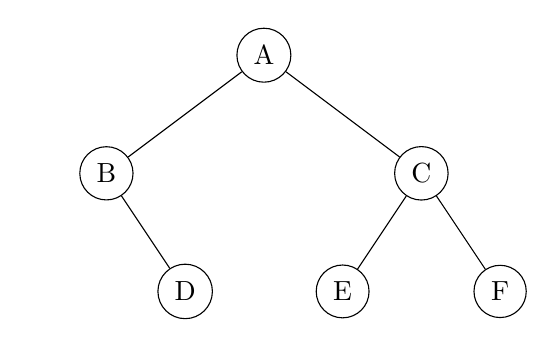
\begin{tikzpicture}[level distance=1.5cm,
        level 1/.style={sibling distance=4cm},
        level 2/.style={sibling distance=2cm},
        every node/.style = {draw, circle}]
        \node {A}
        child { node {B}
            child { edge from parent[draw=none] }
            child { node {D} }
        }
        child { node {C} 
            child { node {E}}
            child { node {F}}
        };
    \end{tikzpicture}
    \label{fig:example_pic}
\end{figure}

The process of doing \textbf{Breadth First Traversal} is: 

\begin{figure}[h]
    \centering
    \raisebox{-2.5em}{\text{front}} \raisebox{-2.5em}{$\rightarrow$}
    \stack{}{}{}{}{A} $\to$
    \stack{}{}{}{C}{B} $\to$
    \stack{}{}{}{D}{C} $\to$
    \stack{}{}{F}{E}{D} $\to$
    \stack{}{}{}{E}{F} $\to$
    \stack{}{}{}{}{F} $\to$
    \stack{}{}{}{}{}
    
    \label{fig:example_sol}
\end{figure}

\pagebreak
\begin{parts}
\part[5] Run \textbf{Pre-order Depth First Traversal} on the tree with root \textbf{A} and draw the whole process in the space below. (Note: it's not required to use all the blank cells.)
\begin{figure}[h]
    \centering 
    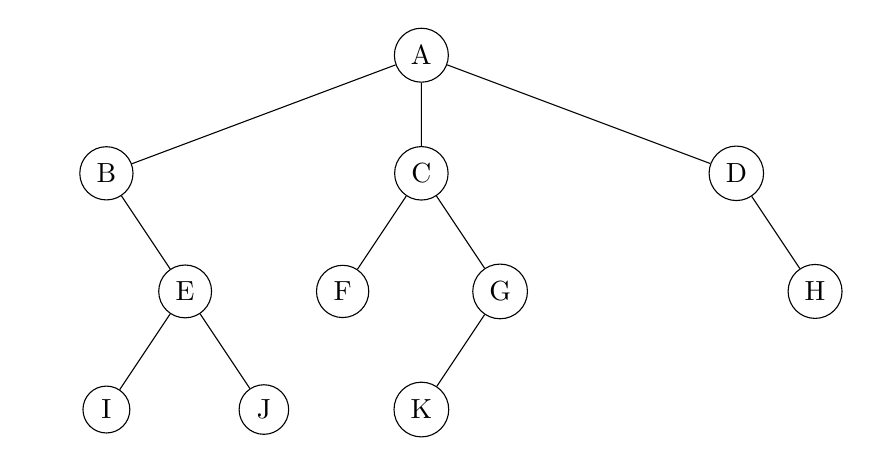
\begin{tikzpicture}[level distance=1.5cm,
        level 1/.style={sibling distance=4cm},
        level 2/.style={sibling distance=2cm},
        level 3/.style={sibling distance=2cm},
        level 4/.style={sibling distance=2cm},
        every node/.style = {draw, circle}]
        \node {A}
        child { node {B}
            child { edge from parent[draw=none] }
            child { node {E} 
                child { node {I} }
                child { node {J} }
            }
        }
        child { node {C} 
            child { node {F}
            }
            child { node {G}
                child { node {K} }
                child { edge from parent[draw=none] }
            }
        }
        child { node {D}
            child { edge from parent[draw=none] }
            child { node {H} }
        };
    \end{tikzpicture}
    \label{fig:example_pic}
\end{figure}
\begin{solution}\\\\
    \begin{minipage}{.14\linewidth}
            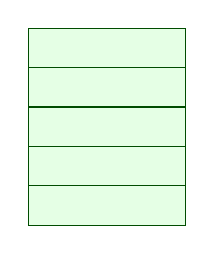
\begin{tikzpicture}[scale=0.5]
                \cell{}
                \cell{}
                \cell{}
                \cell{}
                \cell{}
            \end{tikzpicture}
        \end{minipage}
        $\to$
        \begin{minipage}{.14\linewidth}
            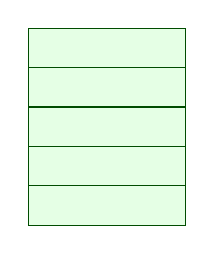
\begin{tikzpicture}[scale=0.5]
                \cell{}
                \cell{}
                \cell{}
                \cell{}
                \cell{}
            \end{tikzpicture}
        \end{minipage}
        $\to$
        \begin{minipage}{.14\linewidth}
            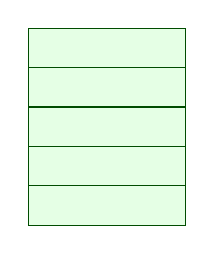
\begin{tikzpicture}[scale=0.5]
                \cell{}
                \cell{}
                \cell{}
                \cell{}
                \cell{}
            \end{tikzpicture}
        \end{minipage}
        $\to$
        \begin{minipage}{.14\linewidth}
            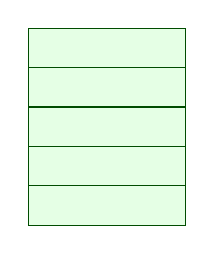
\begin{tikzpicture}[scale=0.5]
                \cell{}
                \cell{}
                \cell{}
                \cell{}
                \cell{}
            \end{tikzpicture}
        \end{minipage}
        $\to$
        \begin{minipage}{.14\linewidth}
            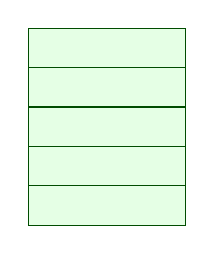
\begin{tikzpicture}[scale=0.5]
                \cell{}
                \cell{}
                \cell{}
                \cell{}
                \cell{}
            \end{tikzpicture}
        \end{minipage}
        $\to$

        \begin{minipage}{.14\linewidth}
            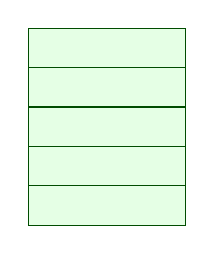
\begin{tikzpicture}[scale=0.5]
                \cell{}
                \cell{}
                \cell{}
                \cell{}
                \cell{}
            \end{tikzpicture}
        \end{minipage}
        $\to$
        \begin{minipage}{.14\linewidth}
            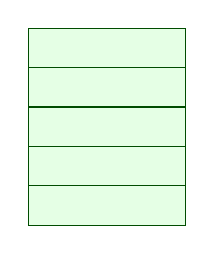
\begin{tikzpicture}[scale=0.5]
                \cell{}
                \cell{}
                \cell{}
                \cell{}
                \cell{}
            \end{tikzpicture}
        \end{minipage}
        $\to$
        \begin{minipage}{.14\linewidth}
            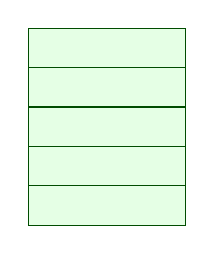
\begin{tikzpicture}[scale=0.5]
                \cell{}
                \cell{}
                \cell{}
                \cell{}
                \cell{}
            \end{tikzpicture}
        \end{minipage}
        $\to$
        \begin{minipage}{.14\linewidth}
            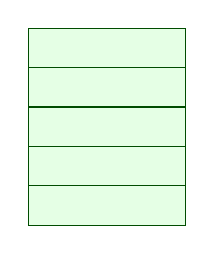
\begin{tikzpicture}[scale=0.5]
                \cell{}
                \cell{}
                \cell{}
                \cell{}
                \cell{}
            \end{tikzpicture}
        \end{minipage}
        $\to$
        \begin{minipage}{.14\linewidth}
            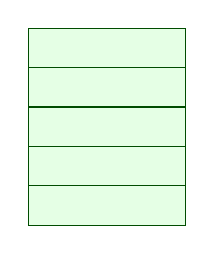
\begin{tikzpicture}[scale=0.5]
                \cell{}
                \cell{}
                \cell{}
                \cell{} 
                \cell{}
            \end{tikzpicture}
        \end{minipage}
        $\to$

        \begin{minipage}{.14\linewidth}
            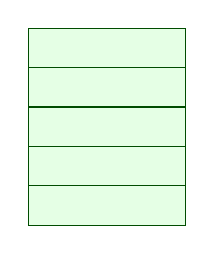
\begin{tikzpicture}[scale=0.5]
                \cell{}
                \cell{}
                \cell{}
                \cell{}
                \cell{}
            \end{tikzpicture}
        \end{minipage}
        $\to$
        \begin{minipage}{.14\linewidth}
            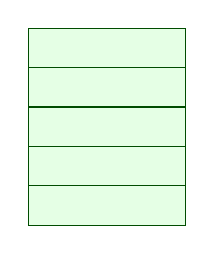
\begin{tikzpicture}[scale=0.5]
                \cell{}
                \cell{}
                \cell{}
                \cell{}
                \cell{}
            \end{tikzpicture}
        \end{minipage}
        $\to$
        \begin{minipage}{.14\linewidth}
            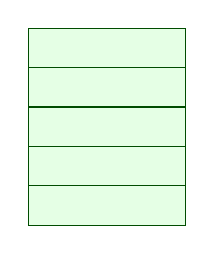
\begin{tikzpicture}[scale=0.5]
                \cell{}
                \cell{}
                \cell{}
                \cell{}
                \cell{}
            \end{tikzpicture}
        \end{minipage}
        $\to$
        \begin{minipage}{.14\linewidth}
            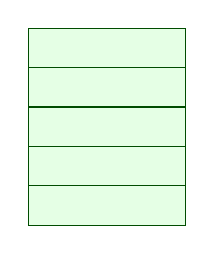
\begin{tikzpicture}[scale=0.5]
                \cell{}
                \cell{}
                \cell{}
                \cell{}
                \cell{}
            \end{tikzpicture}
        \end{minipage}
        $\to$
        \begin{minipage}{.14\linewidth}
            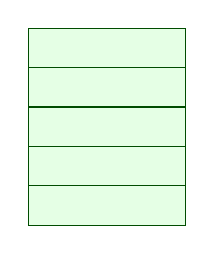
\begin{tikzpicture}[scale=0.5]
                \cell{}
                \cell{}
                \cell{}
                \cell{}
                \cell{}
            \end{tikzpicture}
        \end{minipage}

\end{solution}

\pagebreak
    \part[5]  Run \textbf{Breadth First Traversal} on the tree with root \textbf{A} and draw the whole process in the space below. (Note: it's not required to use all the blank cells.)
    \begin{figure}[h]
    \centering
    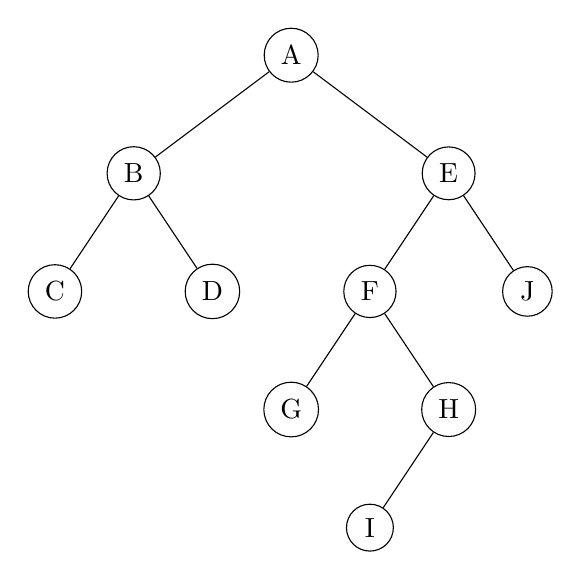
\begin{tikzpicture}[level distance=1.5cm,
        level 1/.style={sibling distance=4cm},
        level 2/.style={sibling distance=2cm},
        level 3/.style={sibling distance=2cm},
        every node/.style = {draw, circle}]
        \node {A}
        child { node {B}
            child { node {C} }
            child { node {D} }
        }
        child { node {E} 
            child { node {F}
                child { node {G}}
                child { node {H}
                    child {node {I}}
                    child { edge from parent[draw=none] }
                }
            }
            child { node {J}}
        };
    \end{tikzpicture}
    \label{fig:example_pic}
\end{figure}
\begin{solution}
\\\\
    \begin{minipage}{.14\linewidth}
            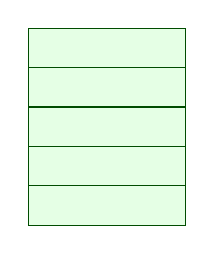
\begin{tikzpicture}[scale=0.5]
                \cell{}
                \cell{}
                \cell{}
                \cell{}
                \cell{}
            \end{tikzpicture}
        \end{minipage}
        $\to$
        \begin{minipage}{.14\linewidth}
            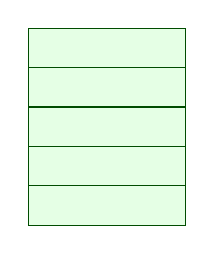
\begin{tikzpicture}[scale=0.5]
                \cell{}
                \cell{}
                \cell{}
                \cell{}
                \cell{}
            \end{tikzpicture}
        \end{minipage}
        $\to$
        \begin{minipage}{.14\linewidth}
            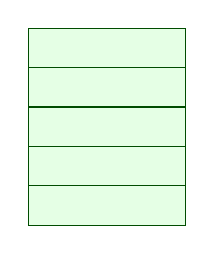
\begin{tikzpicture}[scale=0.5]
                \cell{}
                \cell{}
                \cell{}
                \cell{}
                \cell{}
            \end{tikzpicture}
        \end{minipage}
        $\to$
        \begin{minipage}{.14\linewidth}
            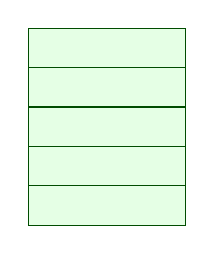
\begin{tikzpicture}[scale=0.5]
                \cell{}
                \cell{}
                \cell{}
                \cell{}
                \cell{}
            \end{tikzpicture}
        \end{minipage}
        $\to$
        \begin{minipage}{.14\linewidth}
            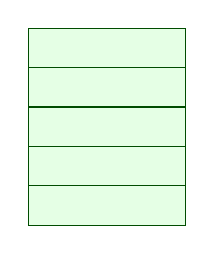
\begin{tikzpicture}[scale=0.5]
                \cell{}
                \cell{}
                \cell{}
                \cell{}
                \cell{}
            \end{tikzpicture}
        \end{minipage}
        $\to$

        \begin{minipage}{.14\linewidth}
            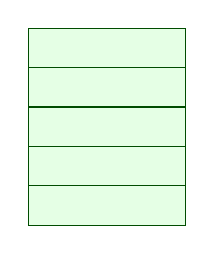
\begin{tikzpicture}[scale=0.5]
                \cell{}
                \cell{}
                \cell{}
                \cell{}
                \cell{}
            \end{tikzpicture}
        \end{minipage}
        $\to$
        \begin{minipage}{.14\linewidth}
            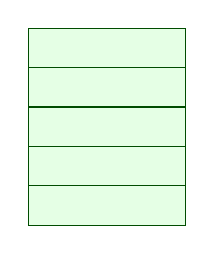
\begin{tikzpicture}[scale=0.5]
                \cell{}
                \cell{}
                \cell{}
                \cell{}
                \cell{}
            \end{tikzpicture}
        \end{minipage}
        $\to$
        \begin{minipage}{.14\linewidth}
            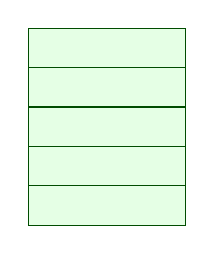
\begin{tikzpicture}[scale=0.5]
                \cell{}
                \cell{}
                \cell{}
                \cell{}
                \cell{}
            \end{tikzpicture}
        \end{minipage}
        $\to$
        \begin{minipage}{.14\linewidth}
            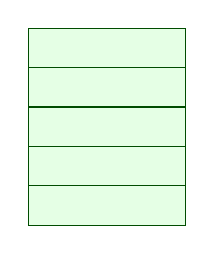
\begin{tikzpicture}[scale=0.5]
                \cell{}
                \cell{}
                \cell{}
                \cell{}
                \cell{}
            \end{tikzpicture}
        \end{minipage}
        $\to$
        \begin{minipage}{.14\linewidth}
            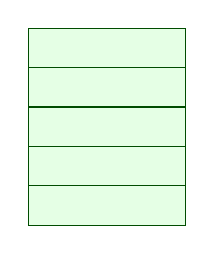
\begin{tikzpicture}[scale=0.5]
                \cell{}
                \cell{}
                \cell{}
                \cell{} 
                \cell{}
            \end{tikzpicture}
        \end{minipage}
        $\to$

        \begin{minipage}{.14\linewidth}
            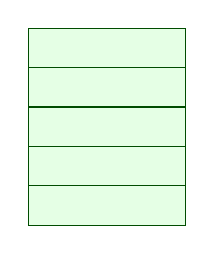
\begin{tikzpicture}[scale=0.5]
                \cell{}
                \cell{}
                \cell{}
                \cell{}
                \cell{}
            \end{tikzpicture}
        \end{minipage}
        $\to$
        \begin{minipage}{.14\linewidth}
            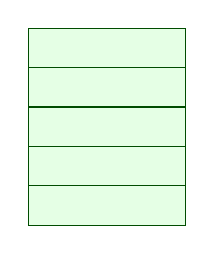
\begin{tikzpicture}[scale=0.5]
                \cell{}
                \cell{}
                \cell{}
                \cell{}
                \cell{}
            \end{tikzpicture}
        \end{minipage}
        $\to$
        \begin{minipage}{.14\linewidth}
            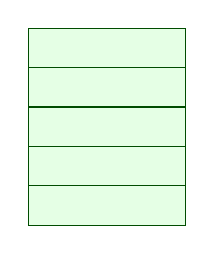
\begin{tikzpicture}[scale=0.5]
                \cell{}
                \cell{}
                \cell{}
                \cell{}
                \cell{}
            \end{tikzpicture}
        \end{minipage}
        $\to$
        \begin{minipage}{.14\linewidth}
            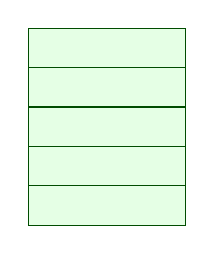
\begin{tikzpicture}[scale=0.5]
                \cell{}
                \cell{}
                \cell{}
                \cell{}
                \cell{}
            \end{tikzpicture}
        \end{minipage}
        $\to$
        \begin{minipage}{.14\linewidth}
            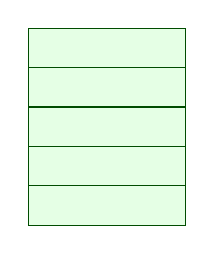
\begin{tikzpicture}[scale=0.5]
                \cell{}
                \cell{}
                \cell{}
                \cell{}
                \cell{}
            \end{tikzpicture}
        \end{minipage}

\end{solution}


\end{parts}

\newpage
\titledquestion{Array Storage}
Unlike arbitrary n-ary trees, binary trees can be easily stored within an array.

\begin{parts}
    \part[6] Complete the code below:
    \begin{verbatim}
    struct BinaryTree {
        int data[SIZE]{};
        
        // Return the index of the root node
        size_t head() {
            return 1;
        }
        
        // Return the index of the left child
        size_t left_child_idx(size_t idx) {
            return ________________;   
            // Fill in the formula for the left child index
        }

        // Return the index of the right child
        size_t right_child_idx(size_t idx) {
            return ________________;   
            // Fill in the formula for the right child index
        }

        // Return the index of the parent node
        size_t parent_idx(size_t idx) {
            return ________________;   
            // Fill in the formula for the parent index
        }
    };
    \end{verbatim}
    \newpage
    \begin{solution}
    \begin{verbatim}
        size_t left_child_idx(size_t idx) {
        
            return ___________________________; 
            
        }
        size_t right_child_idx(size_t idx) {
        
            return ___________________________;   
            
        }
        size_t parent_idx(size_t idx) {
        
            return ___________________________;   
            
        }
    \end{verbatim}
    \end{solution}

    \newpage
    \part[3] To ensure the code functions correctly for all trees with $n$ nodes, what should the minimum \textbf{SIZE} be? You should justify your answer correctly.

    \begin{solution}
    \vspace{8cm}
    \end{solution}

    \part[4] Consider a complete binary tree, the maximum index in this array is 2025, what is the height and number of leaf nodes of this tree? You should justify your answer correctly.

    \begin{solution}
    \vspace{8cm}
    \end{solution}

    
    
\end{parts}



\end{questions}

\end{document}